\documentclass[10pt,twocolumn,letterpaper]{article}

\usepackage{cvpr}
\usepackage{times}
\usepackage{epsfig}
\usepackage{graphicx}
\usepackage{amsmath}
\usepackage{amssymb,bbm,xcolor}
\usepackage[breaklinks=true,bookmarks=false]{hyperref}
\usepackage{lipsum}
\usepackage{listings}
\usepackage{mathtools,eucal}
\usepackage{graphicx}
\graphicspath{ {../data/img/decentralized_stoch/} {../data/img/distributed/}{../data/img/variance_reduced/}}
\usepackage{bbold}
\usepackage{algorithm}
\usepackage[noend]{algpseudocode}
\usepackage{booktabs, multicol, xcolor}
\usepackage[shortlabels]{enumitem}
\usepackage{changepage}
\cvprfinalcopy % *** Uncomment this line for the final submission
\setcounter{page}{1}
\renewcommand{\figurename}{Figure}
\usepackage{amsmath}
\DeclareMathOperator*{\argmax}{arg\,max}
\DeclareMathOperator*{\argmin}{arg\,min}
\DeclareMathAlphabet\mathbfcal{OMS}{cmsy}{b}{n}

\begin{document}
\title{Universal Adversarial Perturbation \\ starring Frank-Wolfe}
\author{Chiara Bigarella\\{\tt\footnotesize Student nr. 2004248}\and Silvia Poletti\\{\tt\footnotesize Student nr. 1239133}\and Gurjeet Singh\\{\tt\footnotesize Student nr. 2004251}\and Francesca Zen\\{\tt\footnotesize Student nr. 2010640}}
\maketitle

% TODO: insert sections here 
\section{Introduction}

\section{Gradient Free Stochastic Frank-Wolfe}
Gradient free optimization algorithms find application in settings where the explicit closed form of the loss function
is not available or the gradient evaluation is computationally prohibitive. A prime example concerns black-box
adversarial attacks on neural networks, where only the model output is known, while the architecture and weights remain
unknown. In fact, gradient free methods exploit just zeroth-order oracle calls (i.e. loss function evaluations) to solve an optimization problem.\\
In particular, this report focuses on zeroth-order Frank-Wolfe algorithms for constrained optimization problems. Unlike
the Projected Gradient Descent (PGD) method that requires expensive projection operations, the Frank-Wolfe framework
provides computational simplicity by making use of instances of linear minimization. Moreover, at each iteration, a
naive zeroth-order analog of PGD takes a step along the estimated gradient aggressively before applying projection,
and since this trajectory might not be a descent direction then the method could suffer from slow convergence.\\
Considering the applications of interest, that are black-box adversarial attacks, a "good enough" feasible solution is
often adequate. Therefore, the use of gradient estimates obtained from zeroth-order information is suitable for performing this task.\\

Let's consider the constrained stochastic optimization problem defined as
\begin{flalign}
	\nonumber
	\mbox{\boldmath$ \delta$}' &= \argmax_{\lVert \mbox{\boldmath$\scriptstyle \delta$}\rVert_{\infty}\leq\varepsilon} \mathbb{E}_{(\mathbf{x},y)\sim \mathcal{P}}[F(\mathbf{x}+\mbox{\boldmath$ \delta$},y)]\\
	& = \argmin_{\lVert \mbox{\boldmath$\scriptstyle \delta$}\rVert_{\infty}\leq\varepsilon} \mathbb{E}_{(\mathbf{x},y)\sim \mathcal{P}}[-F(\mathbf{x}+\mbox{\boldmath$ \delta$},y)]
\end{flalign}
where the couples $(\mathbf{x},y)$ represent the labeled data given in input to the classifier and $F(\mathbf{x},y)$ is
the corresponding loss function. This optimization problem formalizes the procedure to generate a universal adversarial
perturbation that maximizes the loss function on the convex set defined by the infinity norm
$\displaystyle \lVert \mbox{\boldmath$ \delta$}\rVert_{\infty} = \max_{i}|\delta_i|$.\\ According to this formulation,
the adversarial examples are designed to lead to misclassification and the constraint ensures a minimal visual distortion to the human eyes. \\

The zeroth-order optimization is carried out by applying the following biased gradient approximation schemes for $\nabla F(\mathbf{x}_t,y)$:
\begin{itemize}
	\item KWSA:
	\begin{center}
		${\displaystyle\mathbf{g}(\mathbf{x}_t,y) = \sum^{d}_{i=1}\frac{F(\mathbf{x}_t + c_t\mathbf{e}_i,y)-F(\mathbf{x}_t,y)}{c_t}\mathbf{e}_i}$
	\end{center}
	\item RDSA:
	\begin{center}
		${\displaystyle\mathbf{g}(\mathbf{x}_t,y) = \frac{F(\mathbf{x}_t + c_t\mathbf{z}_t,y)-F(\mathbf{x}_t,y)}{c_t}\mathbf{z}_t}$
	\end{center}
	\item I-RDSA:
	\begin{center}
		${\displaystyle\mathbf{g}(\mathbf{x}_t,y) = \frac{1}{m}\sum^{m}_{i=1}\frac{F(\mathbf{x}_t + c_t\mathbf{z}_{i,t},y)-F(\mathbf{x}_t,y)}{c_t}\mathbf{z}_{i,t}}$
	\end{center}
\end{itemize}
where $d$ is the dimension of the optimization problem at hand, $\{\mathbf{e}_i\}_{i=1}^d$ are the canonical basis vectors and $\{\mathbf{z}_{i,t}\}_{i=1}^m\sim\mathcal{N}(0,\mathbb{1}_d)$ are random vectors sampled from the multivariate standard normal distribution.\\
It's easy to see that KWSA is the most query hungry scheme but at the same time is very accurate, while RDSA and I-RDSA are potentially inaccurate but less computationally demanding, and since $m$ is chosen to be independent of $d$ then the query complexity doesn't scale with dimension.\\
Finally, $c_t$ is a time-decaying sequence such that the aforementioned gradient estimators tend to be unbiased for $c_t \rightarrow 0$.\\

In the zeroth-order stochastic Frank-Wolfe framework, the gradient estimate $\mathbf{g}(\mathbf{x}_t,y)$ injects addictional variance to the stochastic counterpart $\nabla F(\mathbf{x}_t,y)$ of the objective function's true gradient $\nabla f(\mathbf{x}_{t},y)$, potentially leading to divergence and exacerbating the fact that the Linear Minimization Oracle (LMO)
\begin{equation}
	\mathbf{v}_t = \argmin_{\mathbf{s}\in\mathit{C}}\langle \mathbf{g}(\mathbf{x}_t,y),\mathbf{s}\rangle	
\end{equation}
is constrained to hold just in expectation.\\ 
To counter this issue, the following gradient smoothing scheme is applied:
\begin{equation}
	\mathbf{d}_{t} = (1-\rho_t)\mathbf{d}_{t-1} + \rho_t\mathbf{g}(\mathbf{x}_t,y)\\
\end{equation}
where $\rho_t$ is a time-decaying sequence and $\mathbb{E}[\lVert\mathbf{d}_{t}-\nabla f(\mathbf{x}_{t},y) \rVert^2]$ can be proved to go to zero asymptotically. Therefore (2) can be rewritten as follows:
\begin{equation}
	\mathbf{v}_t = \argmin_{\mathbf{s}\in\mathit{C}}\langle \mathbf{d}_t,\mathbf{s}\rangle.
\end{equation}
In particular, given the definition of the convex set $\mathit{C}$ as the constraint in (1), the closed-form solution of the LMO is 
\begin{equation}
	\mathbf{v}_t = \argmin_{\lVert \mathbf{s}\rVert_{\infty}\leq\varepsilon}\langle \mathbf{d}_t,\mathbf{s}\rangle= -\varepsilon \:sign(\mathbf{d}_{t}).	
\end{equation}
The final updating rule is
\begin{equation}
	\mathbf{x}_{t+1} = (1-\gamma_t)\mathbf{x}_t + \gamma_t\mathbf{v}_t
\end{equation}
where $\gamma_t\in(0,1]$.
\section{Methods}
Recently, decentralized and distributed settings are getting significant attention due the need to exploit data parallelizability in case of complex model trained on huge data, that typically require a storage that exceeds the machine capacity. In brief, in decentralized setups the devices (or workers) exchange information with a master node, while in distributed setups the devices are connected in a peer-to-peer manner and therefore exchange information only with their neighbors. \\ 
The following optimization algorithm are designed to accomodate distributed data across multiple devices calls.
\subsection{Decentralized Stochastic Gradient Free Frank-Wolfe}
The decentralized architecture is composed of a central node, called master node, and other nodes connected to it but not to each other, called workers.
The workers are connected to the master node to read, write and exchange information.\\
In the Decentralized Stochastic Gradient Free Frank-Wolfe method, the data is spread to $M$ workers and the starting point \mbox{\boldmath$ \delta$}$_{0}$ is initialized to a null $d$-vector.\\
Each worker $i$ computes its local gradient using the I-RDSA scheme and considering a batch of images $\mathbf{x}_i$ and the corresponding labels $\mathbf{y}_i$ from the dataset. Then the workers apply the smoothing scheme (3).\\
When all the workers have finished their tasks, they send their results to the master node, which computes the average of the estimated gradients and send back the new iterate \mbox{\boldmath$ \delta$}$_{t+1}$, obtained from (5) and (6) with $\gamma_t = \frac{2}{t+8}$.\\
When all of the iterations are done, the algorithm returns the hystory of all the perturbations computed by the master node.

\begin{algorithm}
	\caption{Decentralized SGF FW}\label{decentralized} 
	 \textbf{Input} Batches of images $\{\mathbf{x}_i\}_{i=1}^M$, batches of labels $\{\mathbf{y}_i\}_{i=1}^M$, loss function $F$, number of queries $T$, number of workers $M$, image dimension $d$, tolerance $\varepsilon$, number of sampled directions $m$.\\
	 \textbf{Output} Universal perturbation's history.
	\begin{algorithmic}[1]		
		\State Initialize \mbox{\boldmath$ \delta$}$_{0} = \mathbf{0}$.
		\For {$t = 0, \dots, T-1$}
		\State Master node computes parameters required for the computation of the I-RDSA scheme: 
		{\scriptsize\[(\rho_t,c_t)_{I-RDSA} =\bigg(\frac{4}{\big(1+\frac{d}{m}\big)^{1/3}(t+8)^{2/3}}, \frac{2\sqrt{m}}{d^{3/2}(t+8)^{1/3}}\bigg)\]}
		\State Each worker $i$ computes the I-RDSA scheme:\newline Sample $\{\mathbf{z}_{j,t}\}_{j=1}^m \sim\mathcal{N}(0,\mathbb{1}_d)$ \newline
		 \[\mathbf{g}_i = \frac{1}{m} \sum_{j=1}^{m} \frac{F(\mathbf{x}_i + \mbox{\boldmath$ \delta$}_t + c_t\mathbf{z}_{j,t}, \mathbf{y}_i) - F(\mathbf{x}_i + \mbox{\scriptsize\boldmath$ \delta$}_t, \mathbf{y}_i)}{c_t}\mathbf{z}_{j,t}\]
		
		\State Each worker $i$ computes the gradient smoothing scheme:  \[\mathbf{g}_{i,t}= (1- \rho_t)\mathbf{g}_{i,t-1} + \rho_t\mathbf{g}_i.\]
		\State Each worker $i$ pushes $\mathbf{g}_{i,t}$ to the master node.
		\State Master node computes the gradients average:
		\[\mathbf{g}_t = \frac{1}{M} \sum_{i=1}^{M} \mathbf{g}_{i,t}.\]
		\State Master node computes $\mathbf{v}_t = - \varepsilon sign(\mathbf{g}_t)$.
		\State Master node computes \mbox{\boldmath$ \delta$}$_{t+1} = (1-\gamma_t)\mbox{\boldmath$ \delta$}_t + \gamma_t\mathbf{v}_t$ and sends it to all nodes.
		\EndFor

	\end{algorithmic}
\end{algorithm}

\subsection{Decentralized Variance-Reduced Stochastic Gradient Free Frank-Wolfe}
In this section the goal is to solve another special case of (1), that is
\begin{equation}
	\mbox{\boldmath$ \delta$}' = \argmin_{\lVert \mbox{\boldmath$\scriptstyle \delta$}\rVert_{\infty}\leq\varepsilon} \sum_{i=1}^M \sum_{j=1}^n \mathbb{E}_{(\mathbf{x},y)\sim \mathcal{P}_{i,j}}[- F_{i,j}(\mathbf{x}+\mbox{\boldmath$ \delta$},y)].
\end{equation}
The implementation takes into account the SPIDER variance reduction technique, which is built for dynamic tracking, while avoiding excessive querying to oracles and ultimately reducing query complexity.\\
\indent In the Decentralized Variance-Reduced Stochastic Gradient Free Frank-Wolfe method implemented in Algorithm \ref{variance-reduced},
at the beginning of each period, that is when $mod(t,q)=0$ with period parameter $q \in \mathbb{N}_{+}$, each worker employs the KWSA scheme for the computation of its gradient estimation. In all the other cases, each worker selects a mini-batch of local component functions $\{F_{i,j}\}_{j\in S_2}$ and uses the RDSA scheme to estimate and update its gradient. Then, the master node computes the average of the received estimated gradients and calculates the new perturbation using the equation (6) with $\gamma_t = \frac{2}{t+8}$.\\
\indent For what concerns the data, each worker receives the same amount $S_1$ of images (selected to be balanced with respect to the ten classes) and the corresponding labels from the dataset. In particular, the same image is not given to different workers. For both the KWSA and the RDSA schemes, each worker samples a batch of $\frac{S_1}{M}$ images, from the received ones. For the KWSA scheme, this sampling is done $d$ times, one for each component of the gradient.  
\begin{algorithm}
	\caption{Decentralized Variance-Reduced SGF FW}\label{variance-reduced}
	\textbf{Input} Batches of images $\{\mathbf{x}_i\}_{i=1}^M$, batches of labels $\{\mathbf{y}_i\}_{i=1}^M$, loss function $F$, number of queries $T$, number of workers $M$, image dimension $d$, tolerance $\varepsilon$, number of sampled images and labels $S_1$, number of sampled component functions $S_2$, total number of component functions $n$, period $q$.\\
	\textbf{Output} Universal perturbation's history.
	\begin{algorithmic}[1]		
		\State Initialize \mbox{\boldmath$ \delta$}$_{0} = \mathbf{0}$.
		\For {$t = 0, \dots, T-1$}
		\State Master node computes parameters required for the computation of the KWSA and RDSA schemes: 
		{\scriptsize\[\eta_1 =\frac{2}{d^{1/2}(t+8)^{1/3}},\;\;\;\eta_2 =\frac{2}{d^{3/2}(t+8)^{1/3}}\]}
		\State Each worker $i$ computes:
		\If {$mod(t,q)=0$}
		\State For each component $k$ of the gradient, draw $\frac{S_1}{M}$ images $\mathbf{x}'_i$ and the corresponding labels $\mathbf{y}'_i$ from the batches $\mathbf{x}_i$ and $\mathbf{y}_i$, for a total of $\frac{S_1}{M}d$ samples. For $k=1\dots d$ compute \newline
		\[\small \mathbf{e}_k^T\mathbf{g}_i = \frac{1}{n}\sum_{j=1}^{n}\frac{F_{i,j}(\mathbf{x}'_i + \mbox{\boldmath$ \delta$}_t + \eta_1\mathbf{e}_k, \mathbf{y}'_i) - F_{i,j}(\mathbf{x}'_i+\mbox{\boldmath$ \delta$}_t, \mathbf{y}'_i) }{\eta_1} \]
		
		\State Update $\mathbf{g}_{i,t} = \mathbf{g}_i$.
		\Else
		\State Sample $\mathbf{z} \sim\mathcal{N}(0,\mathbb{1}_d)$. Draw $S_2$ component functions and $\frac{S_1}{M}$ images $\mathbf{x}'_i$ and the corresponding labels $\mathbf{y}'_i$ from the batches $\mathbf{x}_i$ and $\mathbf{y}_i$. Then compute
		\[\small \mathbf{g}_i = \frac{1}{|S_2|}\sum_{j\in S_2}\frac{F_{i,j}(\mathbf{x}'_i + \mbox{\boldmath$ \delta$}_t + \eta_2\mathbf{z}, \mathbf{y}'_i) - F_{i,j}(\mathbf{x}'_i+\mbox{\boldmath$ \delta$}_t, \mathbf{y}'_i) }{\eta_2}\mathbf{z} \]
		\[\small-\frac{F_{i,j}(\mathbf{x}'_i + \mbox{\boldmath$ \delta$}_{t-1} + \eta_2\mathbf{z}, \mathbf{y}'_i) - F_{i,j}(\mathbf{x}'_i+\mbox{\boldmath$ \delta$}_{t-1}, \mathbf{y}'_i) }{\eta_2}\mathbf{z} \]
		\State Update $\mathbf{g}_{i,t} = \mathbf{g}_i +\mathbf{g}_{i,t-1} $.
		\EndIf
		\State Each worker $i$ pushes $\mathbf{g}_{i,t}$ to the master node.
		\State Master node computes the gradients average:
		\[\mathbf{g}_t = \frac{1}{M} \sum_{i=1}^{M} \mathbf{g}_{i,t}.\]
		\State Master node computes $\mathbf{v}_t = - \varepsilon sign(\mathbf{g}_t)$.
		\State Master node computes \mbox{\boldmath$ \delta$}$_{t+1} = (1-\gamma_t)\mbox{\boldmath$ \delta$}_t + \gamma_t\mathbf{v}_t$ and sends it to all nodes.
		\EndFor
	\end{algorithmic}
\end{algorithm}

\subsection{Distributed Stochastic Gradient Free Frank-Wolfe}
This section concerns the discussion of the Distributed Stochastic Grandient Free Frank-Wolfe method implemented in Algorithm 3 for the constraint optimization problem (7) in a distributed setup in which the $M$ workers do not have a central coordinator, instead they exchange information in a peer-to-peer manner. The internode communication network used by the workers is modeled as an undirected simply connected graph $G=(V,E)$, with $V=\{1, \dots, M\}$ the set of nodes and $E$ the set of comunication links. Each node communicates and exchanges information with its own neighbors. Given a node $n$, the set $\Omega_n = \{l \in V | (n,l)\in E\}$ indicates its neighborhood and $d_n = |\Omega_n|$ indicates its degree.\\ The $M \times M$ adjacency matrix $\mathbf{A}=[A_{ij}]$ describes the edges of the graph $G$: $A_{ij}=1$ if $(i,j) \in E$ and $A_{ij}=0$ otherwise. The diagonal matrix $\mathbf{D}=diag(d_1 \dots d_M)$ is used to compute the graph Laplacian $\mathbf{L}=\mathbf{D}-\mathbf{A}$. The normalized Laplacian $\mathbfcal{L} = [\mathcal{L}_{ij}]$ is define to be the matrix
\[
\mathcal{L}_{ij}=
\begin{cases}
	1 & \text{if $i=j$ and }d_i\ne0, \\
	-\frac{1}{\sqrt{d_id_j}} & \text{if $i$ and $j$ are adjacent,}\\
	0 & \text{otherwise.}
	
\end{cases}
\]
We can write $\mathbfcal{L} = \mathbf{D}^{-1/2}\mathbf{L}\mathbf{D}^{-1/2}$. The normalized Laplacian $\mathbfcal{L}$ is used to compute the weghted matrix $\mathbf{W} = \mathbb{1}- \mathbfcal{L}$.\\
Unlike the previous algorithms, the perturbation \mbox{\boldmath$ \delta$}$_0$ is initialized as a null $M \times d$ matrix, rather than a vector: this matrix is given in input to each worker, which only considers the rows corresponding to the perturbations computed by its neighbors. This trick simplifies the distributed architecture, without changing the functioning of the algorithm.\\
At every iteration, each worker $i$ exchanges its current iterate with its neighbors and averages the received iterates. Then, each worker $i$ applies the I-RDSA scheme to compute its local gradient estimation $\mathbf{g}_t^i$ and exchanges with the neighbors the vector $\mathbf{G}_t^i$, which is an averaged version of the gradient. Finally, when all the $\mathbf{G}_t^i$ have been calculated, they are involved in a weighted sum computed by each worker.\\
For what said until now, the implementation requires two round of communication: one for the iterates $\bar{\mathbf{x}}_t^i$ and one for the gradients $\bar{\mathbf{g}}_t^i$. The performance depends on how well these vectors are tracked across the network.\\
At the end of the t-th iteration, each worker computes the Frank-Wolfe update of the iterate \mbox{\boldmath$ \delta$}$_{t+1}^i$ using (5) on $\bar{\mathbf{g}}_t^i$ and (6) on $\bar{\mathbf{x}}_t^i$ with $\gamma_t = t^{-1/2}$.\\
\begin{algorithm}
	\caption{Distributed SGF FW}\label{distributed}
	\textbf{Input} Batches of images $\{\mathbf{x}_i\}_{i=1}^M$, batches of labels $\{\mathbf{y}_i\}_{i=1}^M$, loss function $F$, number of queries $T$, number of workers $M$, image dimension $d$, tolerance $\varepsilon$, number of sampled directions $m$, adjacency matrix $\mathbf{A}$, weight matrix $\mathbf{W}$.\\
	\textbf{Output} $\bar{\mbox{\boldmath$ \delta$}}_T^i\;\;\forall i \in \{1\dots M\}$
	\begin{algorithmic}[1]		
		\State For $i=1,\dots, M$ initialize \mbox{\boldmath$ \delta$}$_0^i =\mathbf{0} $ and $\bar{\mathbf{g}}_0^i = \mathbf{0}$
		\For {$t = 1, \dots, T$}
		\State In the first round of communication, each worker $i$ approximates the average iterate: \newline
		\[\bar{\mbox{\boldmath$ \delta$}}_t^i \leftarrow \sum_{j=1}^{M} W_{ij}\mbox{\boldmath$ \delta$}_t^i\]
		\State Each worker $i$ computes the I-RDSA scheme:\newline 
		Sample $\{\mathbf{z}_{j,t}\}_{j=1}^m \sim\mathcal{N}(0,\mathbb{1}_d)$ \newline
		\[\mathbf{g}_t^i = \frac{1}{m} \sum_{j=1}^{m} \frac{F(\mathbf{x}_i + \mbox{\boldmath$ \delta$}_t + c_t\mathbf{z}_{j,t}, \mathbf{y}_i) - F(\mathbf{x}_i + \mbox{\scriptsize\boldmath$ \delta$}_t, \mathbf{y}_i)}{c_t}\mathbf{z}_{j,t}\]
		
		\State  Each worker $i$ computes:
		\[ \mathbf{G}_t^i = \bar{\mathbf{g}}_{t-1}^i + \mathbf{g}_t^i - \mathbf{g}_{t-1}^i \]
		\State In the second round of communication, each worker $i$ approximates the average gradient:
		\[ \bar{\mathbf{g}}_t^i \leftarrow \sum_{j=1}^{M} W_{ij}\mathbf{G}_t^j  \]
		
		\State Each worker $i$ computes $\mathbf{v}_t^i = - \varepsilon sign(\bar{\mathbf{g}}^i_t)$.
		\State Each worker $i$ updates:
		\[\mbox{\boldmath$ \delta$}_{t+1}^i \leftarrow (1-\gamma_t)\bar{\mbox{\boldmath$ \delta$}}_t^i + \gamma_t\mathbf{v}_t^i\]
		\EndFor
		
	\end{algorithmic}
\end{algorithm}
 using $c_t = \frac{2\sqrt{m}}{d^{3/2}(t+8)^{1/3}}$
\section{Experiments}
The data come from the MNIST dataset, containing 60000 train images and 10000 test images from 10 almost balanced classes (arabic numerals). The following simulations generate a universal adversarial perturbation starting from a portion of the MNIST test dataset. Then the perturbation is added to the test images that have been correctly classified by the pre-trained LeNet-5 convolutional neural network, aiming to maximally increase the loss function, and therefore minimize the accuracy.\\
\indent In particular, the perturbation has to inject a minimal visual distortion to the original images and this is ensured by the constraint on the $\ell_{\infty}$ norm in the optimization problem (1). Therefore, the digits in the perturbed images still appear clearly distinguishable to the human eyes, but get misclassified by LeNet-5.\\
\indent 
In the following experiments, the $\ell_{\infty}$ norm of the perturbation is chosen so as not to be higher than $\varepsilon=0.25$.\\

For simplicity, all the algorithms introduced in the previous section have been implemented in a sequential fashion, rather than using a proper distributed architecture. Therefore, the workers do not effectly represent different processors in different machines, but they are just different methods called by the same machine, imitating a distributed setting. Nevertheless, all the algorithms can be easily modified to accomodate a proper distributed architecture by configuring Ray\footnote{Ray: https://github.com/ray-project/ray.} or PySpark\footnote{PySpark: https://spark.apache.org/docs/latest/api/python.} libraries.\\

Again, for simplicity, the algorithms do not involve a normalization technique for the perturbed images and therefore normalization has been applied only after the computation of the universal adversarial perturbation, that is just before the testing of LeNet-5. A possible improvement could be to consider the Box constraint described in \cite{A1}, section V.B.\indent

In addition, a key concept of the Frank-Wolfe theory is the duality gap, that is an upper bound for the primal suboptimality $F(\mathbf{x}_t)-F(\mathbf{x}^*)$ defined as:
\begin{equation}
	\mathcal{G}(\mathbf{x}) =\max_{\mathbf{s}\in\mathit{C}} \langle \nabla F(\mathbf{x}),\mathbf{x}-\mathbf{s}\rangle.
\end{equation}

Therefore, a further improvement of the implementation could be the use of the Frank-Wolfe duality gap as a stopping criterion for the studied algorithms.\\ However, this turned out to be difficult to develop in all of them, since we do not have direct accessibility to the perturbed images from the master node in the decentralized setting. Instead, in the distributed architecture, the presence of a synchronized communication among workers results in a difficult global stopping criteria.
\subsection{Decentralized SGF FW Experiments}
To study the performance of Algorithm \ref{decentralized} we used the 10000 images in the MNIST test set, after normalizing them.\\ We split the digit images by giving 10 samples of each class to our 10 workers.
\begin{figure}[htbp]
	\centering
	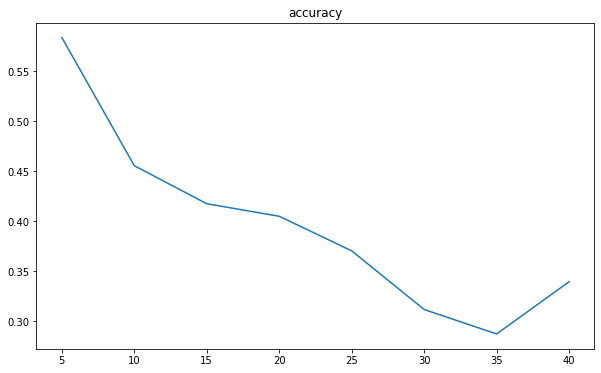
\includegraphics[width=6cm]{accuracy.png}
	\caption{Accuracy of Algorithm \ref{decentralized} with respect to the change on the parameter m.}
	\label{fig:accuracy}
\end{figure}
In Figure \ref{fig:accuracy} we can see a plot in which we represent the behaviour of the Algorithm \ref{decentralized} with respect to the change of the parameter $m$. In particular, we can see that the best value of $m$ who makes the algorithm reaching an accuracy of approximately 20\% is 35, but it is extremely computationally expansive. Fort this reason, we ended up with $m=15$, which is a good compromise between the computation time and the accuracy reached.\\
In our experiments, for each image we estimated its gradient using 20, 50 and 100 queries.\\

\textcolor{gray}{Accuracy error achieved, during the training of the model, the we need to compare the result achieved by testing the model on the whole test set.\\ Notice that the drop of the accuracy, hence the accuracy is discovered already at the 10 epoch/iteration of the algorithms. Comparing the three algorithm is almost the faster one, the competing algorithm in terms of speed convergence of the noise is the distributed.
\\ presence of the pattern in the noise when the accuracy is minimized, more is minimized more the noise the pattern is visible in this algorithms. INstead in the other algorithms the pattern is less visibile e secondo silvia per esempio il variance reduced non presenta un pattern appunto perche il noise e` piu distribuito siccome per la proprieta della varianza considerata nell'algoritmo.
Un piccolo confronto con il guassian noise come fatto nel jupyter sarebbe il top.
}

\begin{figure}
	\centering
	\begin{subfigure}[b]{0.15\textwidth}
		\centering
		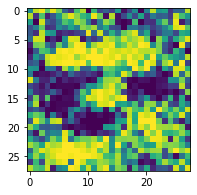
\includegraphics[width=2.5cm]{T20_final.png}
		\caption{}
		\label{fig:decentralized_perturbation_20}
	\end{subfigure}
	\hfill
	\begin{subfigure}[b]{0.15\textwidth}
		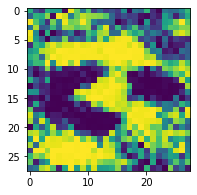
\includegraphics[width=2.5cm]{T50_final.png}
		\caption{}
		\label{fig:decentralized_perturbation_50}
	\end{subfigure}
	\hfill
	\begin{subfigure}[b]{0.15\textwidth}
		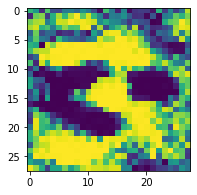
\includegraphics[width=2.5cm]{T100_final.png}
		\caption{}
		\label{fig:decentralized_perturbation_100}
	\end{subfigure}
	\caption{Perturbations of the Decentralized SGF FW algorithm with m=15: \ref{fig:decentralized_perturbation_20} is with T=20, \ref{fig:decentralized_perturbation_50} is with T=50,  \ref{fig:decentralized_perturbation_100} is with T=100.}
	\label{fig:decentralized_perturbations}
\end{figure}
\begin{figure}[h]
	\centering
	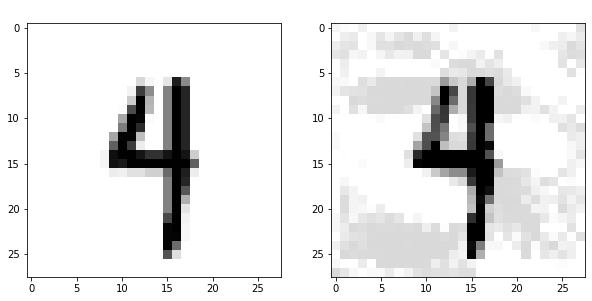
\includegraphics[width=7cm]{image_pertub_T100_final.png}
	\caption{Image of 4 changed to 3 using the best adversarial perturbation generated by the Decentralized Algorithm \ref{decentralized} with a query of 100 and 15 directions.}
	\label{fig:decentralized}
\end{figure}
In Figure \ref{fig:decentralized} we can see an example of the perturbation applyed on an image of the MNIST digits.

\begin{table}[htbp]
	\begin{center}
		\begin{adjustwidth}{-.6cm}{}
			\begin{tabular}{cccc}
				\textbf{Attack} &          20 \textbf{queries} &      50 \textbf{queries} &     100 \textbf{queries} \\
				\midrule
				{\small Decentralized SGF FW}     &    55,25\% &    39,46\% &       36,87\% \\
			\end{tabular}
		\end{adjustwidth}
	\end{center}
	\caption{{\small Summary of $\ell_\infty$ Universal Adversarial Perturbation with $\varepsilon$=0.25. MNIST attack using Decentralized SGF FW. The number of queries is the column denote the nomber of queries used per image.}}
	\label{tab:decentralized}
\end{table}
\subsection{Decentralized Variance-Reduced SGF FW Experiments}
The experiments performed with Algorithm \ref{variance-reduced} were conducted considering $M=5$ workers. Each worker was fed with $S_1=800$ images (80 images per class) from the portion of the MNIST test set that LeNet5 was able to classify correctly. We imposed that the same image could not be assigned to different workers. This aspect was not clearly specified in the original algorithm proposed in \cite{A3}, section VI, in which the authors seem to suggest to use the same $S_1$ images for all the workers. However, the distributed data settings arise from the need of dividing huge datasets into different machines, for simplifying the computational complexity, and therefore we opted for an implementation choice that resulted more coherent with this idea.\\  \indent The number $M$ of workers was halved compared to the one of the previous algorithm and also the other hyperparameters was chosen to be pretty low to reduce a bit the CPU-time consumption. In particular, we set the number of component functions to $n=5$ or $n=10$, the number of sampled components in RDSA to $S_2=3$, the number of queries to $T=20$ and the period parameter to $q=5$ or $q=7$ or $q=9$. With these settings, the algorithm approximatively took between one and four hours to terminate. In fact, the algorithm combines the hungry but accurate queries of KWSA, regulated by the parameter $q$, with the efficient but potentially inaccurate queries of RDSA.\\
\indent In Table \ref{tab:vr} are reported the values of the accuracy reached by LeNet-5 with the adversarial examples obtained using the perturbation generated by Algorithm \ref{variance-reduced}. The attack seems to be more effective as the value of $q$ decreases, i.e. as the KWSA scheme is performed more frequently.\\
\begin{table}[htbp]
	\begin{center}
		\begin{adjustwidth}{-.6cm}{}
			\begin{tabular}{c|cccc}
				\textbf{Attack} &    &      q=5 &      q=7 &     q=10 \\
				\midrule
				{\small Decentralized Variance-}  & n=5   &    92,37\% &    97,43\% &       94,18\% \\
				{\small Reduced SGF FW}     &  n=10&  84,00\% &    93,66\% &       98,99\% \\
			\end{tabular}
		\end{adjustwidth}
	\end{center}
\caption{{\small Summary of $\ell_\infty$ Universal Adversarial Perturbation with $\varepsilon$=0.25. MNIST attacks using Decentralized Variance-Reduced SGF FW. The entries of the table represent the accuracies of LeNet-5 for the three different attacks. For increasing values of $q$ the algorithm performs the KWSA scheme less and less times.}}
	\label{tab:vr}
\end{table}

Figure \ref{fig:vred} compares two adversarial perturbations obtained with same $n$ but different values of $q$. It's clear that the perturbation computed with the lowest $q$ is smoother than the other and less visible to the human eyes.\\
\indent By looking at the colorbar, we can also observe that a higher $q$ results in higher absolute values of the perturbation's components: bright yellow and dark blue pixels indicate values near $\pm\varepsilon$ and are much more frequent in the perturbation computed with the highest $q$.

\begin{figure}[h]
	\begin{subfigure}[b]{0.15\textwidth}
		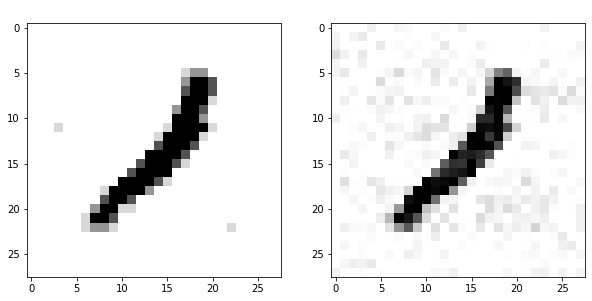
\includegraphics[width=5cm]{image_pertub_q5_n10_final.png}
	\end{subfigure}
	\hspace{2.5cm}
	\begin{subfigure}[b]{0.15\textwidth}
		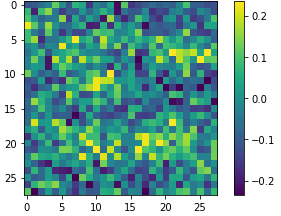
\includegraphics[width=3.08cm]{1.png}
	\end{subfigure}
	\newline
	\centerline{(a)}
	\begin{subfigure}[b]{0.15\textwidth}
		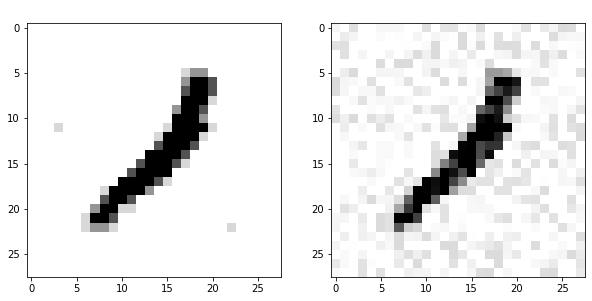
\includegraphics[width=5cm]{image_pertub_q10_n10_final.png}
	\end{subfigure}
	\hspace{2.5cm}
	\begin{subfigure}[b]{0.15\textwidth}
		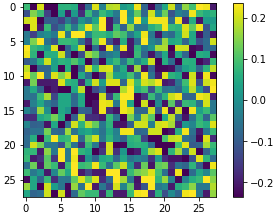
\includegraphics[width=3.07cm]{2.png}
	\end{subfigure}
	\newline
	\centerline{(b)}
	\caption{{\small (a) Adversarial example obtained from Algorithm \ref{variance-reduced} with $n=10$, $q=5$. (b) Adversarial example obtained from Algorithm \ref{variance-reduced} with $n=10$, $q=10$.}  }
	\label{fig:vred}
\end{figure}

\subsection{Distributed SGF FW Experiments}
To test the performance of Algorithm \ref{distributed} we used 10 workers and an adjacecy matrix $A$ given by
\[ A =
\begin{pmatrix}
1& 1& 0& 1& 1& 1& 1& 1& 0& 1\\
1& 1& 1& 0& 1& 1& 1& 0& 1& 1\\
0& 1& 1& 1& 1& 1& 0& 1& 1& 1\\
1& 0& 1& 1& 1& 1& 0& 1& 1& 1\\
1& 1& 1& 1& 1& 1& 1& 0& 1& 1\\
1& 1& 1& 1& 1& 1& 1& 1& 1& 0\\
1& 1& 0& 0& 1& 1& 1& 1& 1& 1\\
1& 0& 1& 1& 0& 1& 1& 1& 1& 1\\
0& 1& 1& 1& 1& 1& 1& 1& 1& 1\\
1& 1& 1& 1& 1& 0& 1& 1& 1& 1
\end{pmatrix}
.\]
We can notice that the diagonal is of ones, this because each node is connected to itself. Our network is composed of
10 nodes and the connectivity of the graph can be know by computing $\Vert W- J \Vert$, where $J= 11^T/10$ and $11^T$
represent a matrix with all entries set to 1. In our case we have a connectivity value of 0.438. We use 15 directions
and test the algorithm for 20, 50 and 100 queries.

\begin{figure}[htbp]
	\centering
	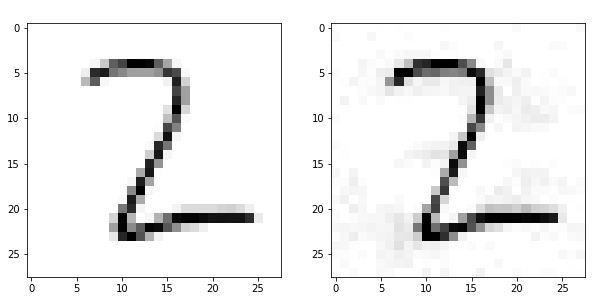
\includegraphics[width=7cm]{image_pertub_T100_final_distr.png}
	\caption{Image of 2 changed to 3 with the adversarial perturbation generated by the Distributed Algorithm \ref{distributed} with 100 queries.}
	\label{fig:distributed}
\end{figure}

\begin{figure}%[htbp]
	\centering
	\begin{subfigure}[b]{0.15\textwidth}
		\centering
		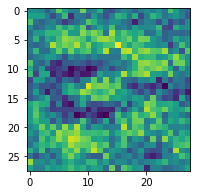
\includegraphics[width=2.5cm]{T20_final_distr.png}
		\caption{}
		\label{fig:decentralized_perturbation}
	\end{subfigure}
	\hfill
	\begin{subfigure}[b]{0.15\textwidth}
		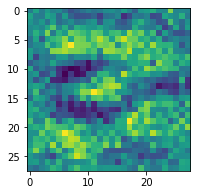
\includegraphics[width=2.5cm]{T50_final_distr.png}
		\caption{}
		\label{fig:variance-reduce_perturbation}
	\end{subfigure}
	\hfill
	\begin{subfigure}[b]{0.15\textwidth}
		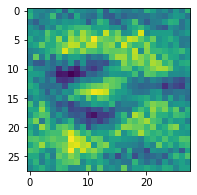
\includegraphics[width=2.5cm]{T100_final_distr.png}
		\caption{}
		\label{fig:distributed_perturbation}
	\end{subfigure}
	\caption{Perturbations of the Distributed SGF FW algorithm: \ref{fig:decentralized_perturbation} is the perturbation with T=20, \ref{fig:variance-reduce_perturbation} is the perturbation with T=50, \ref{fig:distributed_perturbation} is the perturbation with T=100.}
	\label{fig:perturbations}
\end{figure}
\section{Conclusions}
In this report we focused on the problem of producing universal adversarial perturbations by analyzing three
Stochastic Gradient Free Frank-Wolfe algorithms.

First of all, we have shown that the perturbations created by Decentralized (\ref{decentralized}) and Distributed (\ref{distributed})
SGF FW algorithms follow a similar and more clear pattern compared to the Decentralized Variance-Reduced SGF FW
algorithm (\ref{variance-reduced}). In particular, we can clearly see that the reproduced pattern has a 3 shape, which
leads the majority of handwritten digits to be misclassified as 3. This can be explained by the concept of \textit{dominant labels},
mentioned in Section \ref{section:perturb}. In fact, number 3 is a wide number, that covers most of the space in the image. Therefore, a
perturbation with a 3 shape can easily lead to the misclassification of smaller numbers such as 1 and 7, which occupy
less space in the image. On the contrary, the perturbations produced by the Decentralized Variance-Reduced SGF FW algorithm,
don't have a clear pattern and the noise associated with them looks randomly spread.

Secondly, the algorithm that reached better results in terms of misclassification is Algorithm \ref{decentralized},
which lowered the classifier's accuracy to 55\%. In this sense, the worst algorithm was \ref{variance-reduced} since
it was unable to decrease the classifier's accuracy below 84\%.

If we compare the execution time of the three algorithms, we can observe that algorithms \ref{decentralized} and \ref{distributed}
are much faster then algorithm \ref{variance-reduced}. This is due to the fact that algorithm \ref{variance-reduced}
employs KWSA, which is very expensive in terms of CPU time.

Compared to the experiments described in paper \cite{A3}, we obtained slightly higher error rates with algorithm
\ref{decentralized}, while, with algorithm \ref{distributed} , we achieved lower error rates. The latter result can be
explained by the fact that we chose to use I-RDSA with $m=15$ instead of KWSA, to reduce the time complexity of the algorithm,
although KWSA gives a more precise gradient approximation. Furthermore, the distributed setting of algorithm \ref{distributed}
naturally leads to a less precise gradient approximation, due to the fact that each node has access only to the
computations made by its neighbors. Therefore, the choice of a less precise method to compute the gradient, i.e. I-RDSA with a
small value for $m$, make the resulting perturbation less effective. Nevertheless, with this algorithm, we can consider the obtained result satisfying.


% confronto tra i nostri metodi:
% - confronto pattern --> how the noise is spread in the perturbation
% - confronto accuracy --> small accuracy, best algorithm
% - confronto running-time?

% confronto con i risultati del paper:

{\small
	\bibliographystyle{ieee_fullname}
	\bibliography{egbib}
}
\end{document}
